\documentclass[pdf]{beamer}
\mode<presentation>{\usetheme{Luebeck}}

\usepackage{hyperref} % link to tsne.png
\usepackage{wasysym} % smiley face
\usepackage{todonotes}
\usepackage{listings} % display python source
\usepackage{tabularx} % full width tables
\usepackage{tikz}
\usetikzlibrary{fit}

\usepackage{amsmath}
\usepackage{mathtools}
\usefonttheme[onlymath]{serif} % don't use hideous beamer font for math

\title{Sequence to Sequence Learning}
\subtitle{In Natural Language Processing}
\date{May 13, 2017}
\author{Winston Carlile}


%% custom code snippets
\newenvironment{code}{\ttfamily\scriptsize\begin{block}}{\end{block}}
%% toc depth
\setcounter{tocdepth}{1}

\begin{document}
\begin{frame}
  \titlepage
\end{frame}

\begin{frame}{Overview}
  \tableofcontents
\end{frame}
\section{TensorFlow}

\begin{frame}
  \frametitle{Installation}
  \url{https://www.tensorflow.org/install/}
\end{frame}

\subsection{Why?}
\begin{frame}
  \frametitle{Why?}
  Why TensorFlow?
  \begin{itemize}
  \item Expressiveness of Python
  \item Efficiency of optimized CUDA
  \item Scalability\pause
  \item Free \smiley
  \end{itemize}
  \pause
  \url{https://www.tensorflow.org/install/}
\end{frame}

\subsection{How it Works}
\begin{frame}
  \frametitle{How it Works}
  \begin{columns}

    \column{0.4\textwidth}
    \begin{code}{NumPy}
      a = np.random.rand(100,100)\\
      b = np.random.rand(100,100)\\
      np.matmul(a,b)\\
    \end{code}
    \begin{center}
      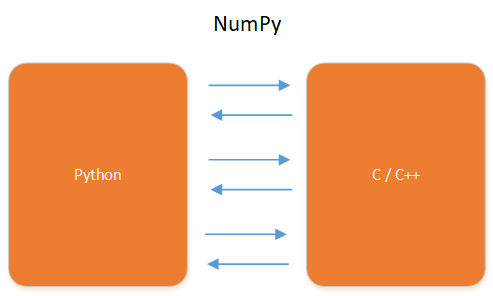
\includegraphics[scale=0.25]{numpy_backend.png}
    \end{center}
    \column{0.6\textwidth}
    \begin{code}{TensorFlow}
      sess = tf.Session()\\
      a = tf.Variable(tf.zeros([100,100]))\\
      b = tf.Variable(tf.zeros([100,100]))\\
      y = tf.matmul(a,b)\\
      sess.run(tf.global\_variables\_initializer())\\
      sess.run(y)\\
    \end{code}
    \begin{center}
      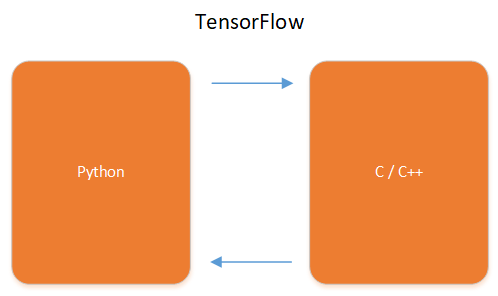
\includegraphics[scale=0.25]{tf_backend.png}
    \end{center}
  \end{columns}
  
\end{frame}

\subsection{Neural Net Crash Course}
\begin{frame}[t]
  \frametitle{Neural Net Crash Course}
  \begin{itemize}
  \item Optimize parameters of function to minimize error
  \item Search parameter space with Gradient Descent Algorithm
  \end{itemize}
  \[ \boldsymbol{\theta}_{t+1} \coloneqq \boldsymbol{\theta}_t-\gamma \frac{dl_n(\boldsymbol{\theta})}{d\boldsymbol{\theta}}\Big|_{\boldsymbol{\theta}_t} \]
\end{frame}

\begin{frame}
  \frametitle{Activation Function Petting Zoo}
  Element-wise nonlinearities
  \begin{itemize}
  \item Sigmoid
    \begin{columns}
      \column{0.4\textwidth}
      \[\boldsymbol{\sigma}(\boldsymbol{\phi})=\frac{1}{1+e^{-\boldsymbol{\phi}}}  \]
      \column{0.3\textwidth} 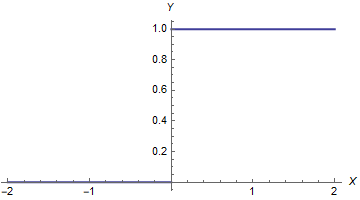
\includegraphics[scale=0.15]{Step.png}
      \column{0.3\textwidth} 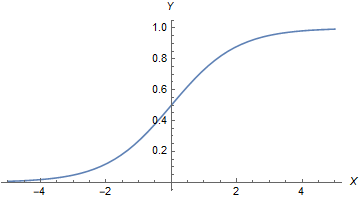
\includegraphics[scale=0.15]{Sigmoid.png}
    \end{columns}
  \item Gaussian Radial Basis
    \begin{columns}
      \column{0.4\textwidth}
      \[\boldsymbol{\psi}(\boldsymbol{\phi})=\exp(-\boldsymbol{\phi}\odot\boldsymbol{\phi}) \]
      \column{0.6\textwidth} 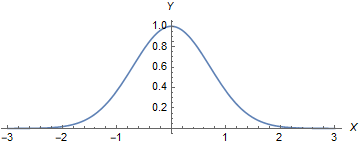
\includegraphics[scale=0.15]{Gaussian.png}
    \end{columns}
  \item Softplus
    \begin{columns}
      \column{0.4\textwidth}
      \[
        \boldsymbol{q}(\boldsymbol{\phi})=\log(1+e^{\boldsymbol{\phi}}) \]
      \column{0.3\textwidth} 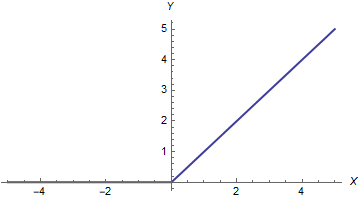
\includegraphics[scale=0.15]{Rectified.png}
      \column{0.3\textwidth} 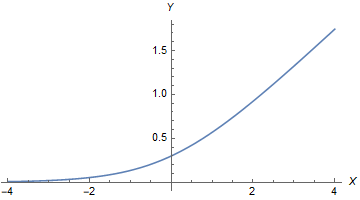
\includegraphics[scale=0.15]{Softplus.png}
    \end{columns}
  \end{itemize}
  
\end{frame}

\begin{frame}
  \frametitle{Loss Function Petting Zoo}
  % $l_n(\boldsymbol{\theta})= $Prediction error using parameters
  % $\boldsymbol{\theta}$\\
  % $\ddot{\boldsymbol{y}}(\boldsymbol{\theta},\boldsymbol{s}_i) = $ the prediction of
  % the network given input $\boldsymbol{s}_i$ $\boldsymbol{\theta}$
  \begin{itemize}
  \item Continuous Output (regression)
    \[ l_n(\boldsymbol{\theta}) = \frac{1}{n}\sum_{i=1}^{n} |\boldsymbol{y}_i
      -\boldsymbol{\ddot{y}}(\boldsymbol{\theta},\boldsymbol{s}_i)|^2
    \]
  \item Binary Output (classification)
    \[ l_n(\boldsymbol{\theta}) = -\frac{1}{n}\sum_{i=1}^{n}
      \big[\boldsymbol{y}_i\log(\ddot{\boldsymbol{y}}(\boldsymbol{\theta},\boldsymbol{s}_i))
      + (1-\boldsymbol{y}_i)\log(1-\ddot{\boldsymbol{y}}(\boldsymbol{\theta},\boldsymbol{s}_i))\big]
    \]
    \begin{columns}
      \column{0.5\textwidth}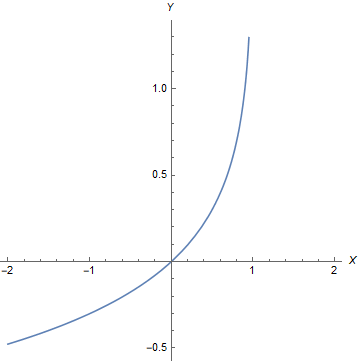
\includegraphics[scale=0.20]{-logx.png}
      \column{0.5\textwidth}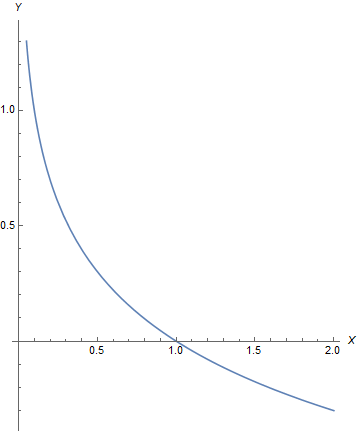
\includegraphics[scale=0.17]{-log1-x.png}
    \end{columns}
  \end{itemize}
\end{frame}

\subsection{Example}
\begin{frame}
  \frametitle{MNIST}
  \begin{code}{Clone the Demo}
    \$ git clone https://github.com/WChurchill/seq2seq\_workshop.git\\
    \$ cd seq2seq\_workshop/code\\
    \$ python mnist.py\\
  \end{code}
  or,\\
  \footnotesize\texttt{<path-to-tensorflow>/tensorflow/examples/tutorials/mnist/mnist.py}
\end{frame}

\section{Word Embeddings}
\subsection{Idea}
\begin{frame}[t]
  \frametitle{Word Embeddings}
  \begin{itemize}
  \item Pretrain using unsupervised learning
  \item Train a small network to recognize valid n-grams
  \end{itemize}
  \begin{center}
    %% define layersep for tikz diagrams
    \def\layersep{1.5cm}
    \textnormal{}\begin{tikzpicture}[shorten >=1pt,->,draw=black!50, node distance=\layersep]
      \tikzstyle{every pin edge}=[<-,shorten <=1pt];
      \tikzstyle{neuron}=[circle,fill=black!25,minimum size=8pt,inner sep=0pt];
      \tikzstyle{input neuron}=[neuron, fill=green!50];
      \tikzstyle{output neuron}=[neuron, fill=red!50];
      % \tikzstyle{embedding}=[rect, draw=black];
      \tikzstyle{annot} = [text centered];


      % Draw the input layer nodes
      \foreach \name / \y in {0,...,14}
      % This is the same as writing \foreach \name / \y in {1/1,2/2,3/3,4/4}
      \node[input neuron] (I-\name) at (0.6*\y - 1,0) {};

      \node[draw=black,fit=(I-0)(I-1)(I-2),pin={below:do}] {};
      \node[draw=black,fit=(I-3)(I-4)(I-5),pin={below:not}] {};
      \node[draw=black,fit=(I-6)(I-7)(I-8),pin={below:like}] {};
      \node[draw=black,fit=(I-9)(I-10)(I-11),pin={below:green}] {};
      \node[draw=black,fit=(I-12)(I-13)(I-14),pin={below:eggs}] {};
      % \draw[annot, below of: rectan] {I};
      % Draw the hidden layer nodes
      % \foreach \name / \y in {1,...,5}
      % \path[yshift=0.5cm]
      % node[hidden neuron] (H-\name) at (\layersep,-\y cm) {};

      % Draw the output layer node
      \node[output neuron,pin={[pin edge={->},distance={0.1cm}]above: Valid}] (O) at (3.25, \layersep) {};

      % Connect every node in the input layer with every node in the
      % hidden layer.
      % \foreach \source in {1,...,4}
      % \foreach \dest in {1,...,5}
      % \path (I-\source) edge (H-\dest);

      % Connect every node in the hidden layer with the output layer
      \foreach \source in {0,...,14}
      \path (I-\source) edge (O);

      % Annotate the layers
      % \node[annot,above of=H-1, node distance=1cm] (hl) {Hidden layer};
      % \node[annot,left of=hl] {Input layer};
      \node[annot,left of=O,node distance=3cm] {$\ddot{y} (\boldsymbol{ W },\boldsymbol{ s })\equiv\frac{1}{1+e^{-\boldsymbol{Ws}}} $};
    \end{tikzpicture}
  \end{center}
\end{frame}

\subsection{Code}
\begin{frame}
  \frametitle{Code}
  Try it!
  \begin{code}{Run word2vec.py}
    \$ python word2vec\_basic.py\\
    \$ ls\\
    tsne.png\\
    
  \end{code}
\end{frame}
\subsection{Results}
\begin{frame}
  \frametitle{Results}
  \href{tsne.png}{tsne.png}
  \begin{center}
    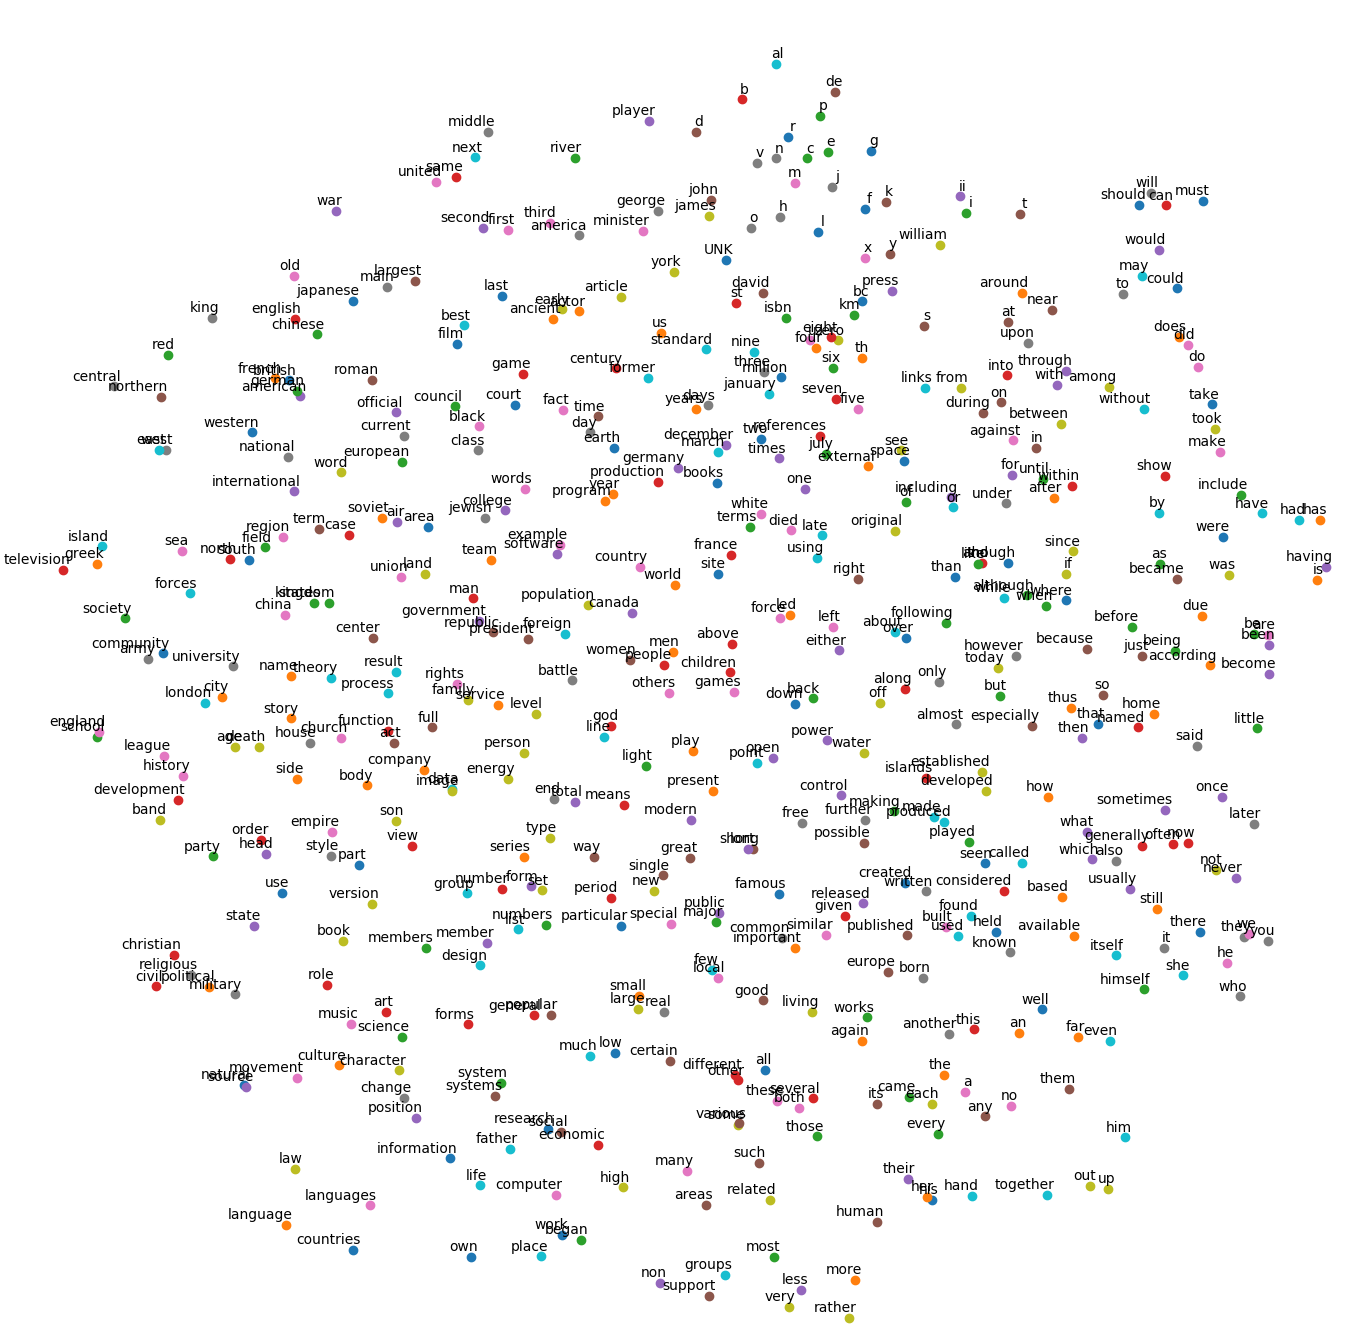
\includegraphics[scale=0.2]{tsne.png}
  \end{center}
  
\end{frame}

\section{BPTT}
\subsection{Problem}
\begin{frame}
  
  \frametitle{But What About Sequences?}
  \begin{itemize}
  \item Matrix dimensions are fixed
  \item Architecture is static
  \item How do we make networks with variable length inputs?
  \item How do we make networks with variable length outputs?
  \end{itemize}
  \pause
  \begin{alertblock}{Bad Idea}
    Find maximum length of input \& output vectors during preprocessing
  \end{alertblock}
  
\end{frame}


\begin{frame}[t]
  \frametitle{Recurrent Neural Networks}
  \begin{itemize}
  \item Networks that feed into themselves
  \item Hidden units remember by self-activation
  \end{itemize}

  %% define layersep for tikz diagrams
  \def\layersep{1.5cm}
  \begin{center}
    \textnormal{}\begin{tikzpicture}[shorten >=1pt,->,draw=black!50, node distance=\layersep]
      \tikzstyle{every pin edge}=[<-,shorten <=1pt];
      \tikzstyle{neuron}=[circle,fill=black!25,minimum size=17pt,inner sep=0pt];
      \tikzstyle{input neuron}=[neuron, fill=green!50];
      \tikzstyle{hidden neuron}=[neuron, fill=blue!50];
      \tikzstyle{output neuron}=[neuron, fill=red!50];
      % \tikzstyle{embedding}=[rect, draw=black];
      \tikzstyle{annot} = [text centered];


      % Draw the input layer nodes
      \foreach \name / \y in {1,...,4}{
        % This is the same as writing \foreach \name / \y in {1/1,2/2,3/3,4/4}
        \node[input neuron] (I-\name) at (\y,0) {};
      }
      % \draw[annot, below of: rectan] {I};
      % Draw the hidden layer nodes
      \foreach \name / \y in {1,...,5}{
        \path[xshift=-0.5cm] 
        node[hidden neuron] (H-\name) at (\y cm,\layersep) {};
      }
      
      % Draw the output layer node
      \node[output neuron,above of=H-3] (O) {};

      % Connect every node in the input layer with every node in the
      % hidden layer.
      \foreach \source in {1,...,4}{
        \foreach \dest in {1,...,5}{
          \path (I-\source) edge (H-\dest);
        }
      }

      % Connect every node in the hidden layer with the output layer
      \foreach \source in {1,...,5}{
        \path (H-\source) edge (O);
        \path (H-\source) edge [draw=black,max distance = 5mm,looseness=7,out=45, in=135] (H-\source) ;
      }
      % Annotate the layers
      \node[annot,right of=H-5, node distance=2cm] (hl) {$ \boldsymbol{h}_t(\boldsymbol{W},\boldsymbol{s},\boldsymbol{h}_{t-1}) $};
      % \node[annot,left of=hl] {Input layer};
      % \node[annot,left of=O,node distance=3cm] {$\ddot{y} (\boldsymbol{ W },\boldsymbol{ s })\equiv\frac{1}{1+e^{-\boldsymbol{Ws}}} $};
    \end{tikzpicture}
  \end{center}
\end{frame}

\begin{frame}
  \frametitle{Backpropogation Through Time}
  \begin{columns}
    \column{0.3\textwidth}
    \[ D\equiv [\boldsymbol{S}_1, \boldsymbol{S}_2, \ldots, \boldsymbol{S}_n] \]
    \[ \boldsymbol{S}_i\equiv [\boldsymbol{s}_{i1}, \boldsymbol{s}_{i2}, \ldots, \boldsymbol{s}_{iT_i}] \]
    \column{0.7\textwidth}
    \begin{center}
      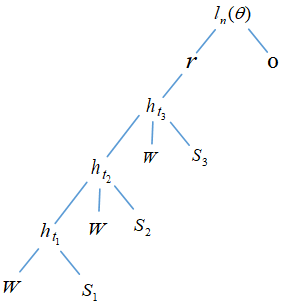
\includegraphics[scale=0.8]{functional_hierarchy.png}
    \end{center}
  \end{columns}
\end{frame}

\subsection{Encoding}

\begin{frame}
  \frametitle{Expanded Network Diagram}
  %% define layersep for tikz diagrams
  \def\layersep{1cm}
  \begin{center}
    \textnormal{}\begin{tikzpicture}[shorten >=1pt,->,draw=black!50,node distance=\layersep]
      \tikzstyle{every pin edge}=[<-,shorten <=1pt];
      \tikzstyle{neuron}=[circle,fill=black!25,minimum size=12pt,inner sep=0pt];
      \tikzstyle{input neuron}=[neuron, fill=green!50];
      \tikzstyle{hidden neuron}=[neuron, fill=blue!50];
      \tikzstyle{output neuron}=[neuron, fill=red!50];
      % \tikzstyle{embedding}=[rect, draw=black];
      \tikzstyle{annot} = [text centered, node distance=.5cm];


      % Draw the input layer\nodes
      \foreach \name / \y in {1,...,3}
      % This is the same as writing \foreach \name / \y in {1/1,2/2,3/3,4/4}
      \node[hidden neuron] (I0-\name) at (\y,0) {};

      % \draw[annot, below of: rectan] {I};
      % Draw the hidden layer\nodes
      \foreach \name / \y in {1,...,5}{
        \path[xshift=0.5cm]
        node[hidden neuron] (H0-\name) at (\y cm,\layersep) {};
      }

      \foreach \name / \y in {1,...,5}{
        \path[xshift=3cm]
        node[hidden neuron] (H1-\name) at (\y cm,2*\layersep) {};
      }
      
      \foreach \name / \y in {1,...,2}{
        \path[xshift=5.5cm]
        node[hidden neuron] (H2-\name) at (\y cm,3*\layersep) {};
      }
      
      % Draw the output layer nodes
      \foreach \name / \y in {1,...,4}{
        \path[xshift=4.5cm]
        node[output neuron] (O-\name) at (\y cm, 4*\layersep) {};
      }

      % Connect every\node in the input layer with every\node in the
      % hidden layer.
      \foreach \source in {1,...,3}
      \foreach \dest in {1,...,2}
      \path (I-\source) edge (H0-\dest);

      \foreach \source in {1,...,5}
      \foreach \dest in {1,...,2}
      \path (H0-\source) edge (H1-\dest);

      \foreach \source in {1,...,5}
      \foreach \dest in {1,...,2}
      \path (H1-\source) edge (H2-\dest);
      
      
      % Connect every\node in the hidden layer with the output layer
      \foreach \source in {1,...,2}
      \foreach \dest in {1,...,4}
      \path (H2-\source) edge (O-\dest);
      
      % Annotate the layers
      \node[annot,below of=I-2] {what};
      \node[annot,below of=H0-4] {is};
      \node[annot,below of=H1-4] {love};
    \end{tikzpicture}
    \newline Input sequence is encoded as a finite-length
    vector
  \end{center}


\end{frame}
\subsection{Decoding}
\begin{frame}
  \frametitle{Decoding}
  \def\layersep{1cm}
  \begin{center}
    \textnormal{}\begin{tikzpicture}[shorten >=1pt,->,draw=black!50,node distance=\layersep]
      \tikzstyle{every pin edge}=[<-,shorten <=1pt];
      \tikzstyle{neuron}=[circle,fill=black!25,minimum size=12pt,inner sep=0pt];
      \tikzstyle{input neuron}=[neuron, fill=green!50];
      \tikzstyle{hidden neuron}=[neuron, fill=blue!50];
      \tikzstyle{output neuron}=[neuron, fill=red!50];
      % \tikzstyle{embedding}=[rect, draw=black];
      \tikzstyle{annot} = [text centered, node distance=.5cm];


      % Draw the input layer\nodes
      \foreach \name / \y in {1,...,4}{
        % This is the same as writing \foreach \name / \y in {1/1,2/2,3/3,4/4}
        \path[xshift=0cm]
        node[output neuron] (I0-\name) at (\y,0) {};
      }

      % \draw[annot, below of: rectan] {I};
      % Draw the hidden layer\nodes
      \foreach \name / \y in {1,...,2}{
        \path[xshift=1cm]
        node[hidden neuron] (H0-\name) at (\y cm,\layersep) {};
      }

      \foreach \name / \y in {1,...,5}{
        \path[xshift=0.5cm]
        node[hidden neuron] (H1-\name) at (\y cm,2*\layersep) {};
      }
      
      \foreach \name / \y in {1,...,5}{
        \path[xshift=3cm]
        node[hidden neuron] (H2-\name) at (\y cm,3*\layersep) {};
      }
      
      % Draw the output layer nodes
      \foreach \name / \y in {1,...,5}{
        \path[xshift=5.5cm]
        node[hidden neuron] (O-\name) at (\y cm, 4*\layersep) {};
      }

      % Connect every\node in the input layer with every\node in the
      % hidden layer.
      \foreach \source in {1,...,4}
      \foreach \dest in {1,...,2}
      \path (I-\source) edge (H0-\dest);

      \foreach \source in {1,...,2}
      \foreach \dest in {1,...,5}
      \path (H0-\source) edge (H1-\dest);

      \foreach \source in {4,...,5}
      \foreach \dest in {1,...,5}
      \path (H1-\source) edge (H2-\dest);
      
      
      % Connect every\node in the hidden layer with the output layer
      \foreach \source in {4,...,5}
      \foreach \dest in {1,...,5}
      \path (H2-\source) edge (O-\dest);
      
      % Annotate the layers
      \node[annot,above of=H1-2] {baby};
      \node[annot,above of=H2-2] {dont};
      \node[annot,above of=O-2] {hurt};
    \end{tikzpicture}
    \newline Output sequence is a repeated projection of the encoded vector
  \end{center}
\end{frame}

\begin{frame}
  \frametitle{Vanishing Gradient}
  \begin{itemize}
  \item Gradient is disproportionately small in bottom layers
  \item Output layers receive most of the blame
  \item Performs poorly on long sequences
  \end{itemize}
\end{frame}

\section{LSTM}

\begin{frame}
  \frametitle{Long Short-Term Memory}
  \begin{itemize}
  \item Information highway through time
  \item Network learns explicitly what to remember
  \end{itemize}
\end{frame}
\subsection{Anatomy}
\begin{frame}[t]
  \frametitle{Anatomy of an LSTM Cell}
  \begin{center}
    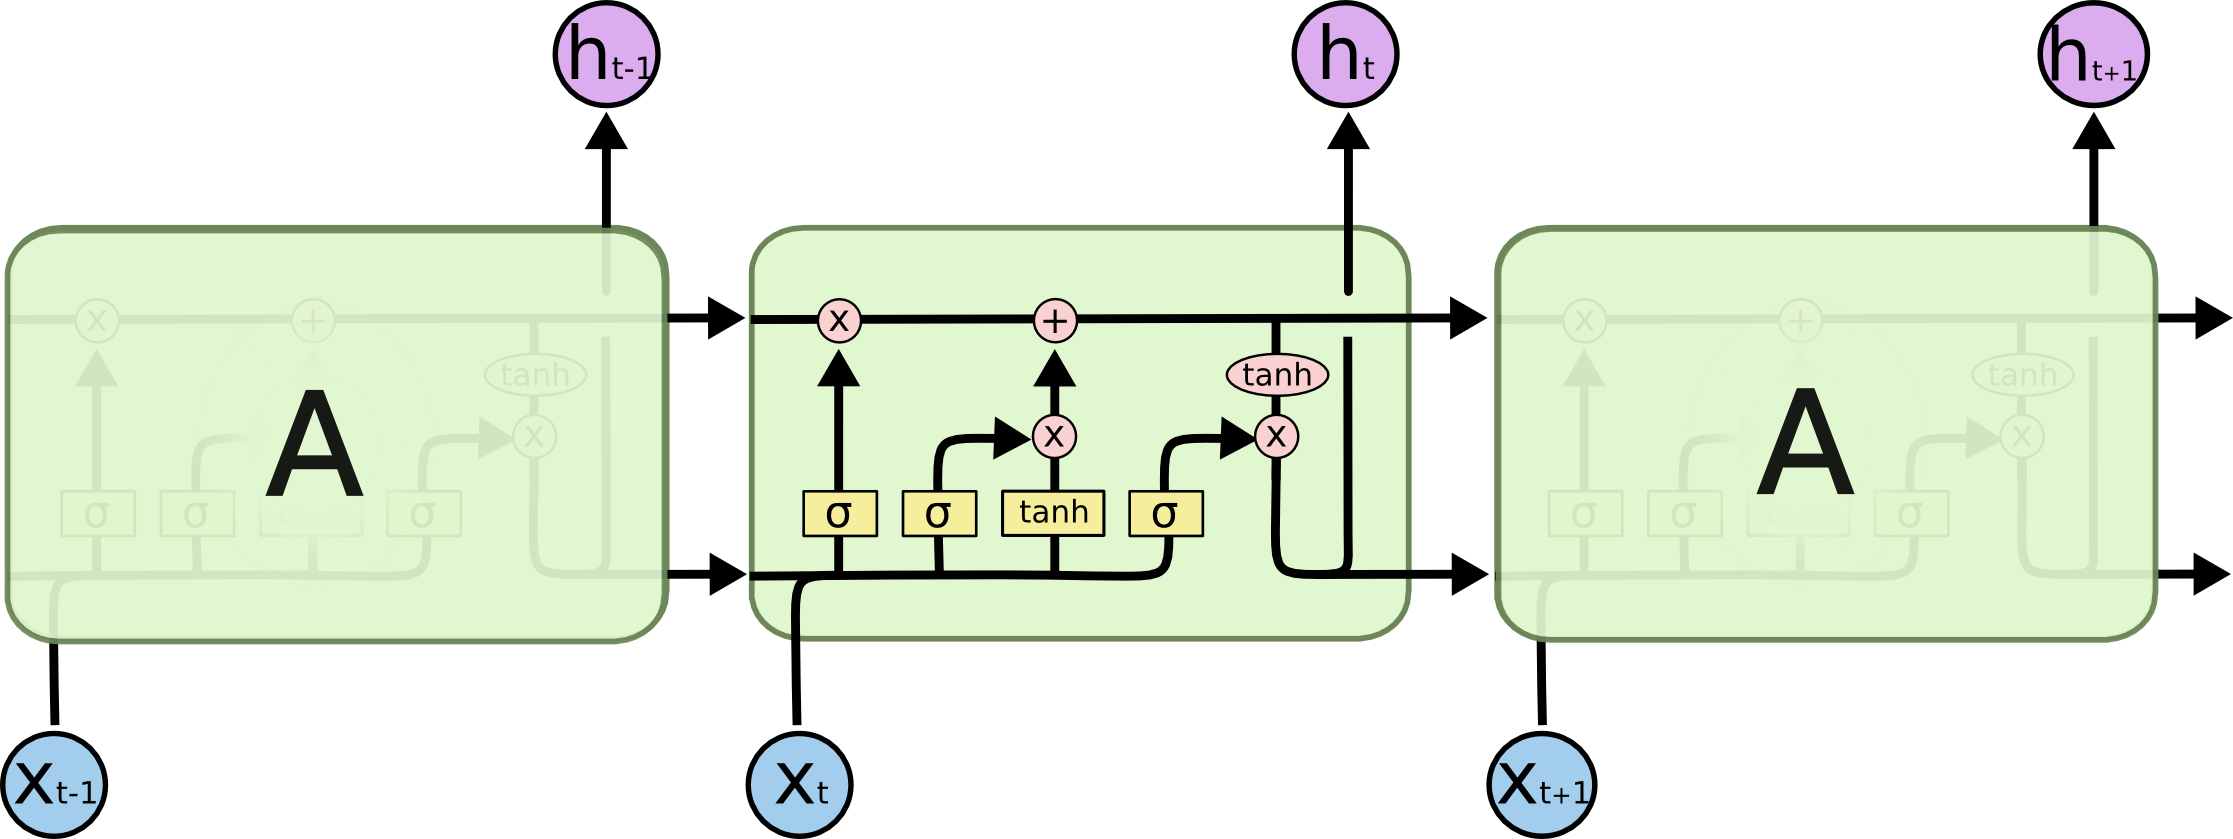
\includegraphics[scale=0.4]{LSTM3-chain.png}
  \end{center}
  \footnotesize  \url{http://colah.github.io/posts/2015-08-Understanding-LSTMs/}
\end{frame}

\begin{frame}
  \frametitle{Code}
  \begin{code}{rnn\_tutorial.py}
    lstm = tf.contrib.rnn.BasicLSTMCell(<num\_units>)\\
    state = tf.zeros([<batch size>, <lstm state size>])
  \end{code}
\end{frame}

\begin{frame}
  \frametitle{Even More Improvements!}
  Some questions you might have:
  \begin{itemize}
  \item What's the difference between the cell state and hidden state?
  \item What's the difference between remembering new information and
    forgetting the old?
  \item Why are the gates blind to the cell state?
  \end{itemize}
\end{frame}
\subsection{GRU}
\begin{frame}
  \frametitle{Gated Recurrent Units}
  \begin{center}
    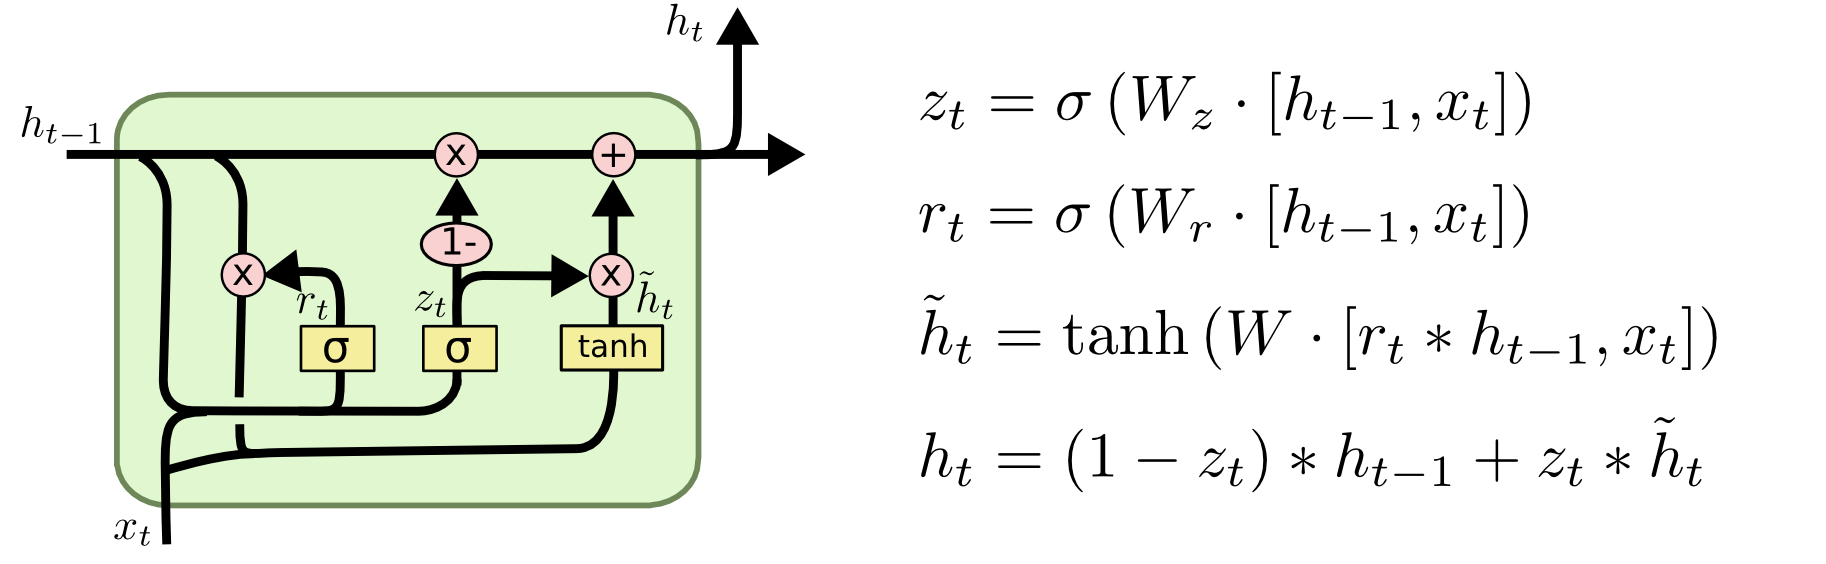
\includegraphics[scale=0.4]{LSTM3-var-GRU.png}\\
  \end{center}
  \footnotesize  \url{http://colah.github.io/posts/2015-08-Understanding-LSTMs/}
\end{frame}
\subsection{Code}
\begin{frame}
  \frametitle{Code}
  \begin{code}{Try It! (if you have 6 hours or a beefy GPU)}
    \$ python translate.py\\
    downloading dataset... \# very large file\\
    \# wait 3 hours depending on internet quality\\
    \# dataset is downloaded\\
    \# begin preprocessing\\
    \# 3 more hours\\
  \end{code}
  \pause
  \begin{alertblock}{ERROR!}
    Your model is incorrect
  \end{alertblock}
\end{frame}
\subsection{Stacking LSTM Cells}
\begin{frame}{Stacking LSTM Networks}
  \begin{code}{rnn\_tutorial.py}
    lstm = tf.contrib.rnn.BasicLSTMCell(<num\_units>)\\
    stacked\_lstm = tf.contrib.rnn.MultiRNNCell([lstm] * <num\_layers>)
  \end{code}
  \begin{center}
    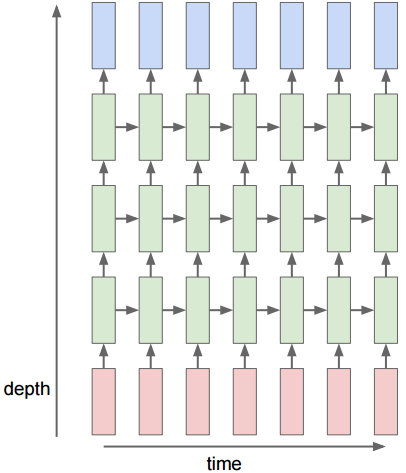
\includegraphics[scale=0.2]{RNN_Stacking.png}\\
  \end{center}
  \footnotesize \url{https://leonardoaraujosantos.gitbooks.io/artificial-inteligence/content/recurrent_neural_networks.html}
\end{frame}

\begin{frame}
  \frametitle{Other Applications in NLP}
  \begin{itemize}
  \item Speech recognition
  \item Conversational Agents
  \item Automated Summarization
  \end{itemize}
\end{frame}

\begin{frame}
  \frametitle{What Now?}
  Amazon Web services
  \begin{itemize}
  \item Discount supercomputer
  \item Gigabit internet speed
  \item Harness the scalability of tensorflow
    \pause
  \item Additional setup
  \end{itemize}
\end{frame}

\section*{}
\begin{frame}
  \begin{center}
    \Large{Questions and Discussion}
  \end{center}
\end{frame}

\end{document}
%%% Local Variables:
%%% mode: latex
%%% TeX-master: t
%%% End:
